% \begin{frame}{Co dalej?}

%     \textcolor{cfblue}{Hipoteza (Bang-Jensen i Hell, 1990)} \\
%     Niech \(H\) będzie spójnym grafem bez źródeł i ujść. Jeśli \(H\) ma homomorfizm do cyklu, to~problem CSP\((H)\) jest w klasie P, wpp CSP\((H)\) jest NP-zupełny.

%     W nieskończoności:
%     \begin{figure}
%     \centering
%         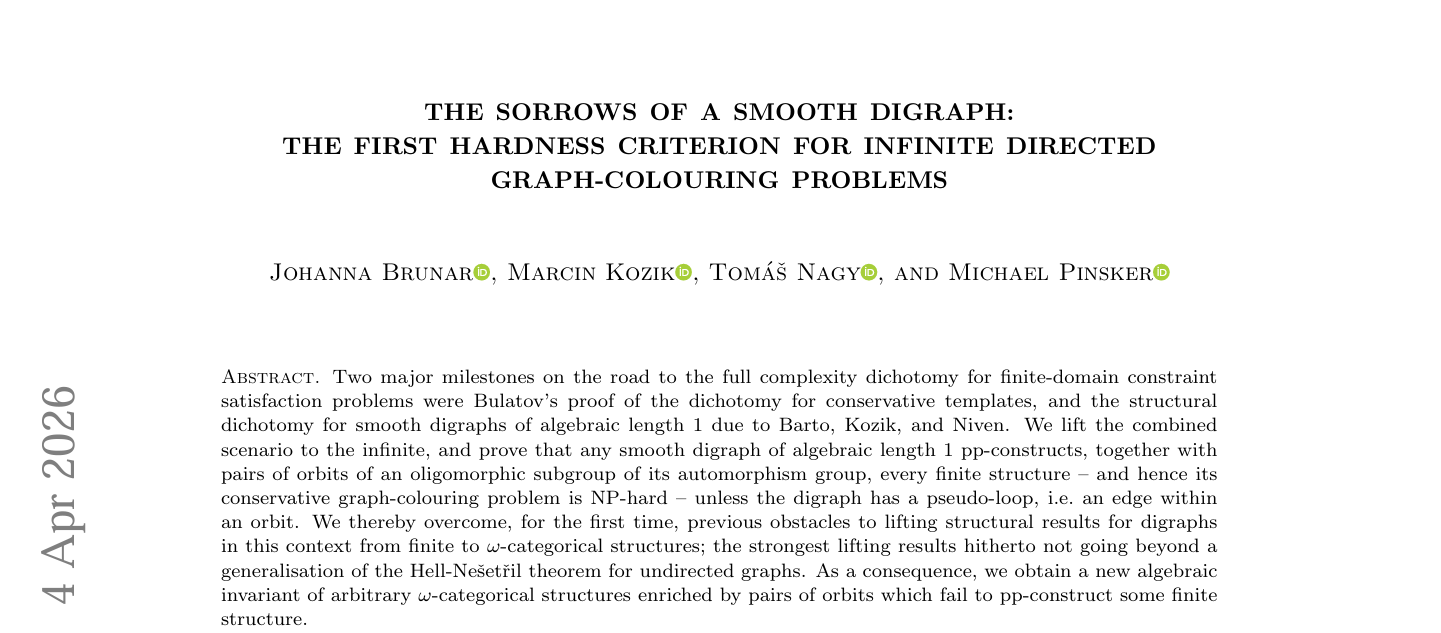
\includegraphics[width=0.85\linewidth]{img/paper.png}
%     \end{figure}
    
% \end{frame}

% -----------------------------------------------------------

\begin{frame}{Postępy}

    \begin{figure}
        \centering
        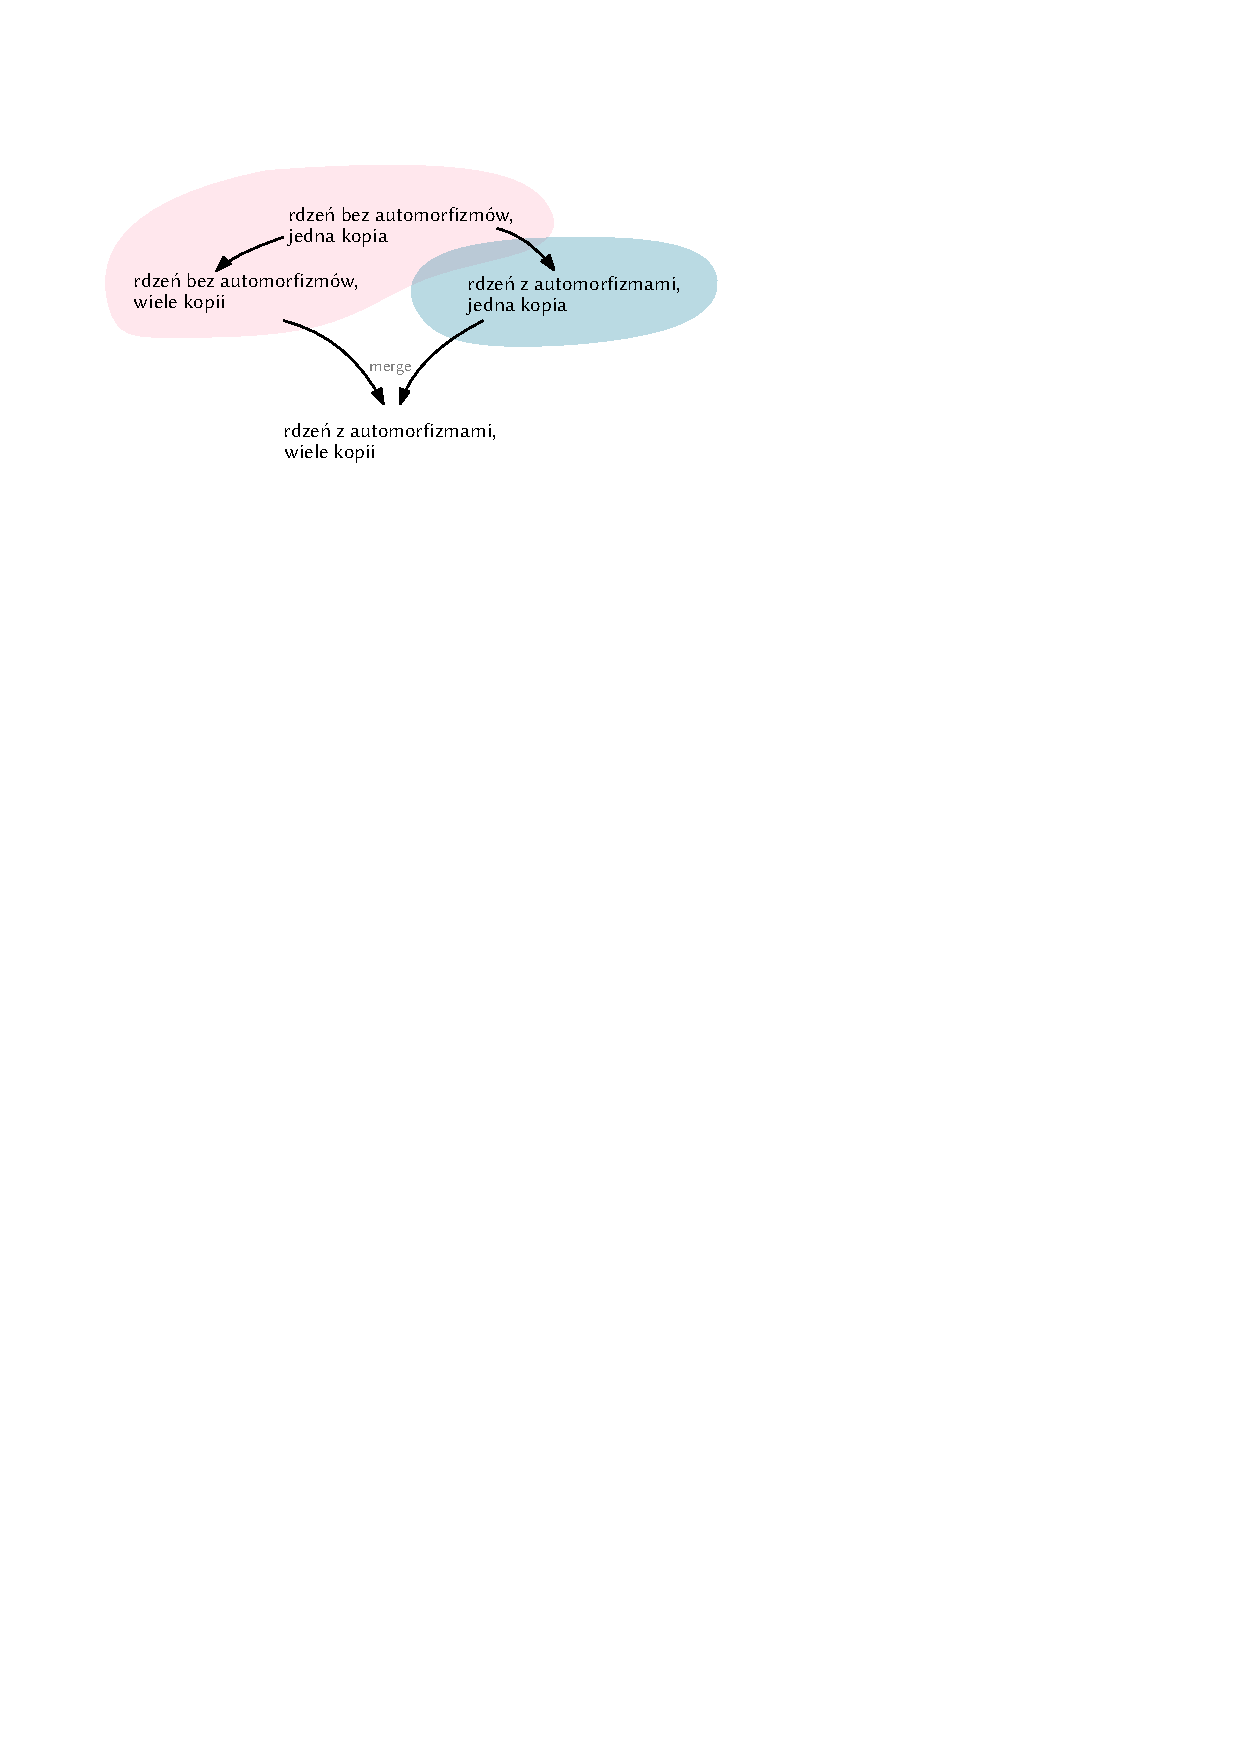
\includegraphics{img/progress.pdf}
    \end{figure}

\end{frame}

% -----------------------------------------------------------

\begin{frame}{Polimorfizmy}
    n-arny polimorfizm grafu \(f\) to funkcja \(V^n\to V\) taka, że:
    \[\forall{(u_1,v_1),\dots,(u_n,v_n)\in E(G)} \Longrightarrow (f(u_1,\dots,u_n), f(v_1,\dots,v_n))\in E(G)\]
    \begin{figure}
        \centering
        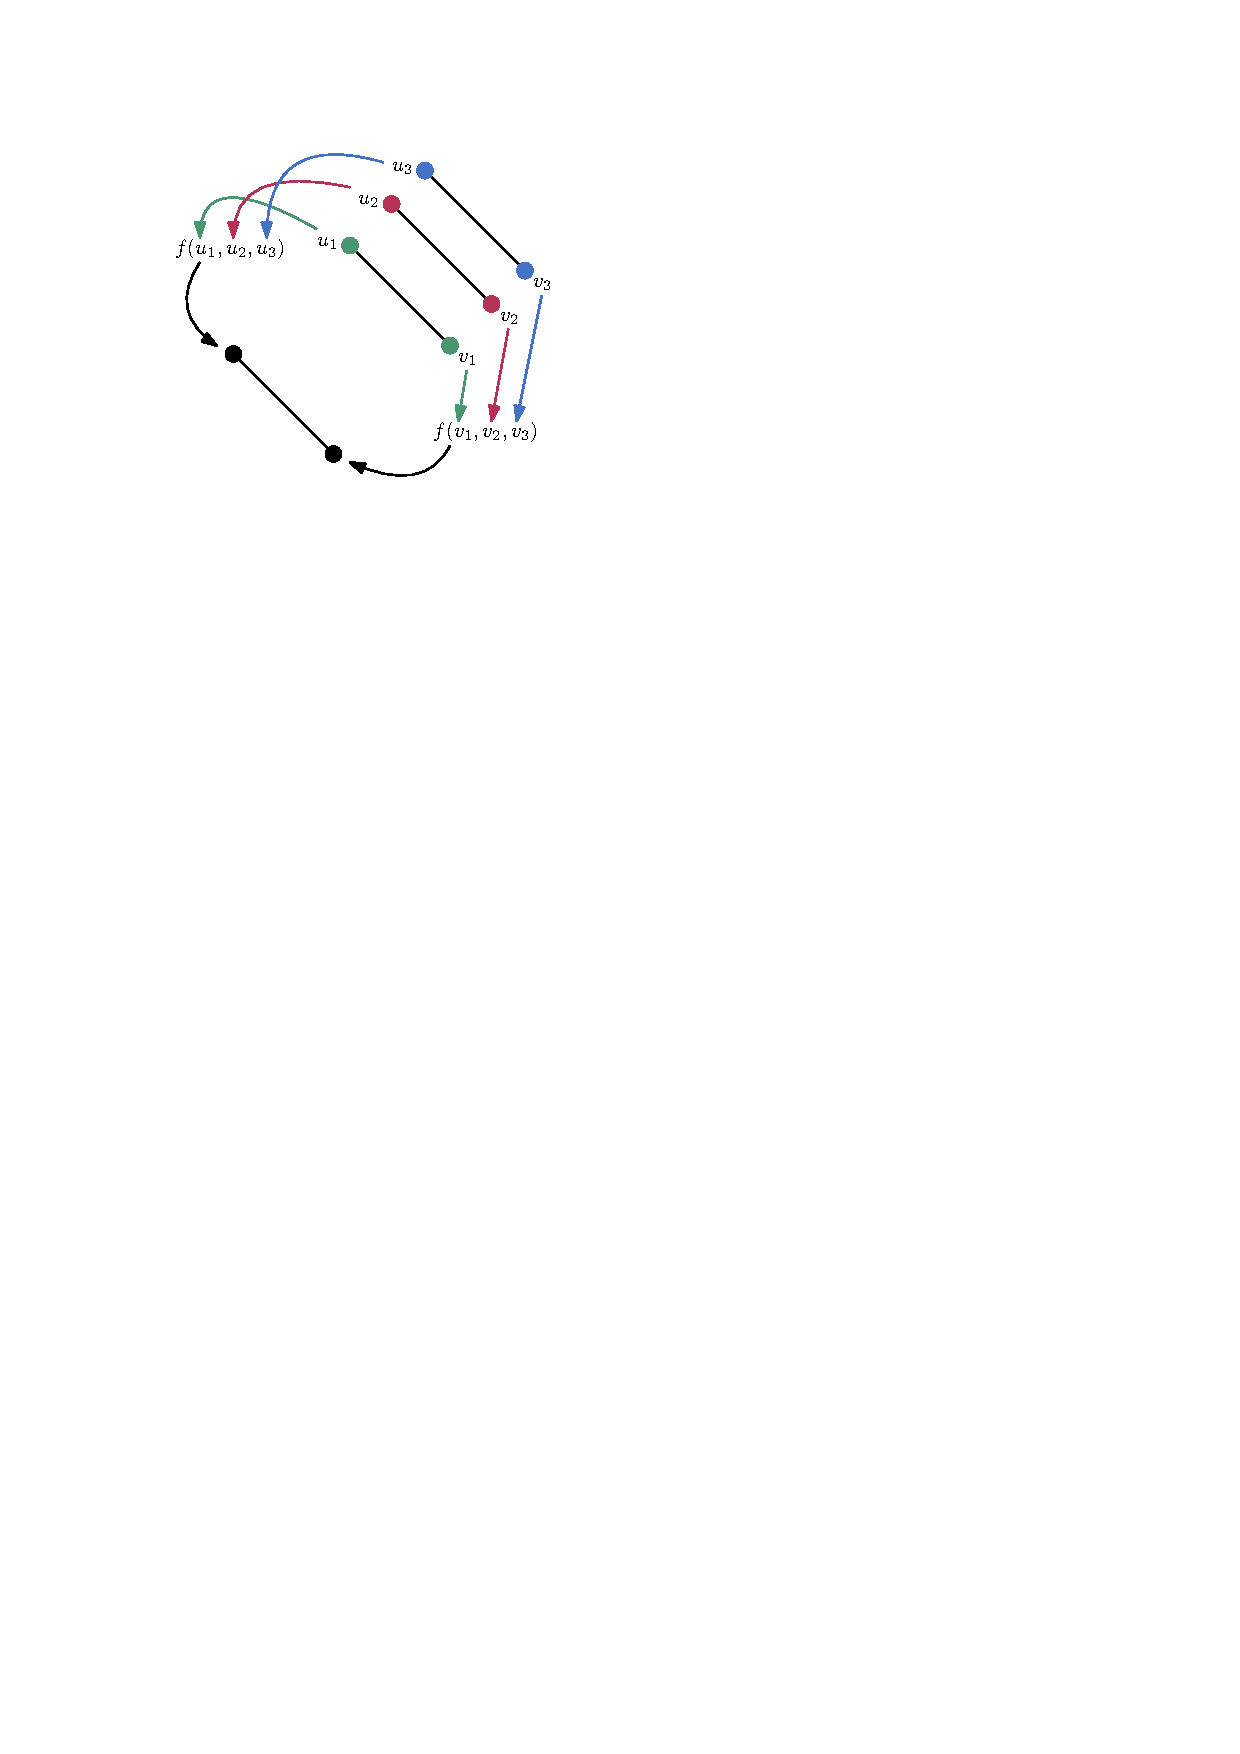
\includegraphics[width=0.4\linewidth]{fig/polymorphism.pdf}
    \end{figure}
\end{frame}

% -----------------------------------------------------------

\begin{frame}{Co dalej}

    \textcolor{cfblue}{Dychotomia CSP (Bulatov, Zhuk; 2017)} \\
    Każdy szablon albo pp-konstruuje wszystkie skończone struktury, albo jest niezmienniczy względem pewnego polimorfizmu \(s\), który spełnia:
    \vspace{-1em}
    \[ s(x,y,z,x) = s(y,x,y,z) \qquad \text{(tożsamość Siggersa)} \]

    \vspace{0.75em}
    \pause
    \textcolor{cfblue}{Dychotomia dla nieskończonych CSP* (Barto, Pinsker)} \\
    Każdy nieskończony szablon albo pp-konstruuje wszystkie skończone struktury, \linebreak albo posiada jednoargumentowe polimorfizmy \(u, v\) oraz 6-arny polimorfizm \(s\) taki, że
    \vspace{-1em}
    \[ u s(x,y,x,z,y,z) = v s(y,x,z,x,z,y) \]
    \\\vspace{-1em}
    dla wszystkich \(x,y,z\).

    {\tiny *~Uproszczenie}

\end{frame}